% !TEX root = task-3-7.tex
% Editable task bank. Append new BankTask blocks at the end of the document.
\documentclass[12pt,a4paper]{article}
\usepackage{physics-textbook}
\usepackage{graphicx,needspace}
\usetikzlibrary{decorations.pathmorphing}
\newif\ifShowSolutions
\ifdefined\TutorEdition
  \ShowSolutionstrue
\else
  \ShowSolutionsfalse % Change to \ShowSolutionstrue to display solutions.
\fi
\newcounter{banktask}
\newsavebox{\BankTaskBox}
\newcommand{\BankTaskContent}[3]{%
  \noindent\textbf{\thebanktask.}\quad #2\par
  \ifShowSolutions
    \Needspace{50mm}% Keep the solution heading with its opening text or diagram.
    #3\par
    \ifdefined\TutorEdition
      \ifcsname TutorSource#1\endcsname
        \nopagebreak\smallskip{\small\csname TutorSource#1\endcsname\par}%
      \fi
    \fi
  \fi
}
\newcommand{\BankTask}[3]{%
  \refstepcounter{banktask}\par\medskip
  \sbox{\BankTaskBox}{\begin{minipage}{\linewidth}%
    \BankTaskContent{#1}{#2}{#3}\end{minipage}}%
  \ifdim\dimexpr\ht\BankTaskBox+\dp\BankTaskBox\relax>\dimexpr\textheight-20mm\relax
    \Needspace{35mm}\BankTaskContent{#1}{#2}{#3}%
  \else
    \Needspace{\dimexpr\ht\BankTaskBox+\dp\BankTaskBox\relax}%
    \noindent\usebox{\BankTaskBox}\par
  \fi
  \medskip
}
\begin{document}
\BookSubsection{3.7}{Конденсатор. Энергия электрического поля}


% Source 7D4F20: https://ege.fipi.ru/bank/questions.php?search=1&proj=BA1F39653304A5B041B656915DC36B38&qid=7D4F20
\BankTask{7D4F20}{
Необходимо экспериментально изучить зависимость заряда, накопленного конденсатором, от сопротивления резистора. Какие две схемы следует использовать для проведения такого исследования?

\begin{center}
\begin{tikzpicture}[book diagram, x=1cm, y=1cm]
\foreach \x/\n/\source/\res in {0/1/{\mathcal{E},r}/{R},2.6/2/{2\mathcal{E},2r}/{2R},5.2/3/{2\mathcal{E},r}/{2R},7.8/4/{\mathcal{E},2r}/{R},10.4/5/{\mathcal{E},r}/{2R}} {
\begin{scope}[shift={(\x,0)}]
\node at (0.65,-0.55) {\n)};
\draw (0,0)--(0,1.8)--(0.57,1.8);
\draw (0.72,1.8)--(1.35,1.8)--(1.35,0)--(0.73,0);
\draw (0.57,1.57)--(0.57,2.03);
\draw (0.72,1.68)--(0.72,1.92);
\node[anchor=south west] at (0.67,1.97) {$\source$};
\draw (0,0.83)--(0.3,0.83);
\draw (0.3,0.68) rectangle (1.04,0.98);
\draw (1.04,0.83)--(1.35,0.83);
\fill (0,0.83) circle (0.035);
\fill (1.35,0.83) circle (0.035);
\node[anchor=south] at (0.67,1.01) {$\res$};
\draw (0,0)--(0.57,0);
\draw (0.57,-0.24)--(0.57,0.24);
\draw (0.73,-0.24)--(0.73,0.24);
\node[anchor=south west] at (0.76,0.04) {$C$};
\end{scope}
}
\end{tikzpicture}
\end{center}
}{
\smallskip\noindent\textbf{Решение от GPT}\par
Менять нужно только сопротивление резистора, сохраняя одинаковыми ЭДС источника, его внутреннее сопротивление и ёмкость конденсатора. Этому условию соответствуют схемы 1 и 5: сопротивления равны соответственно $R$ и $2R$, а остальные параметры совпадают. В схеме 2 изменены ЭДС и внутреннее сопротивление, в схеме 3 — ЭДС, в схеме 4 — внутреннее сопротивление относительно схемы 1. После установления режима $q=CU=\dfrac{C\mathcal{E}R_{\text{рез}}}{R_{\text{рез}}+r}$. Ответ: 15.
}

% Source 9327: https://phys-ege.sdamgia.ru/problem?id=9327
\BankTask{9327}{
\begin{center}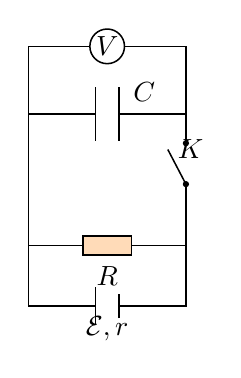
\begin{tikzpicture}[>=stealth,line width=.55pt]\draw(0,0)--(0,3.3)--(2,3.3)--(2,2.07) (2,1.55)--(2,0)--(1.15,0) (.85,0)--(0,0) (0,2.44)--(.85,2.44) (1.15,2.44)--(2,2.44) (0,.77)--(2,.77);\draw(.85,-.24)--(.85,.24) (1.15,-.15)--(1.15,.15) (.85,2.1)--(.85,2.78) (1.15,2.1)--(1.15,2.78);\fill(2,2.07)circle(.04) (2,1.55)circle(.04);\draw(2,1.55)--(1.77,1.99)node[right]{$K$};\node at(1.47,2.72){$C$};\node[below]at(1,0){$\mathcal E,r$};\draw[fill=white](1,3.3)circle(.22)node{$V$};\draw[fill=orange!28](0.69,0.65)rectangle(1.31,0.89);\node[above]at(1,0.89){$$};\node[below]at(1,.63){$R$};\end{tikzpicture}\end{center}Опираясь на законы физики, найдите показание идеального вольтметра в схеме, представленной на рисунке, до замыкания ключа К и опишите изменения его показаний после замыкания ключа К. Первоначально конденсатор не заряжен.
}{
\smallskip\noindent\textbf{Решение}\par
$1$.  Начальное показание вольтметра равно нулю, после замыкания ключа показания вольтметра будут увеличиваться, пока не достигнут максимального значения, которое не будет меняться со временем.
$2$.  Вольтметр соединен параллельно с конденсатором, поэтому его показания равны напряжению на конденсаторе. Вначале конденсатор не заряжен $( q_1=0 ) ,$ поэтому напряжение на нем $U_1= \frac{q_1}{C} =0,$ и показания вольтметра равны нулю.
$3$.  После замыкания конденсатор будет заряжаться, и, так как $U= \frac{q}{C} ,$ показания вольтметра будут увеличиваться. Когда конденсатор полностью зарядится, ток через него не течет, а течет только через резистор. Сила тока в цепи станет постоянной и согласно закону Ома для полной цепи $I= \frac{\varepsilon}{R + r} .$ Напряжение на конденсаторе и резисторе $U=IR$ и не будет меняться со временем. Поэтому показания вольтметра тоже перестанут изменяться.
}

% Source 41154: https://phys-ege.sdamgia.ru/problem?id=41154
\BankTask{41154}{
\begin{center}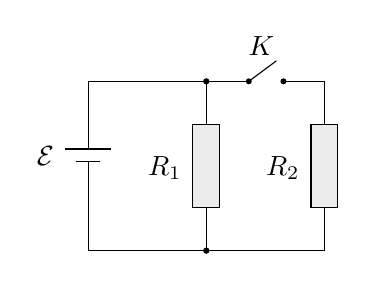
\begin{tikzpicture}[>=stealth]

\draw (0,0)--(3,0)--(3,.55) (3,1.6)--(3,2.15)--(2.48,2.15) (2.04,2.15)--(0,2.15)--(0,1.29) (0,1.13)--(0,0);
\draw (-.29,1.29)--(.29,1.29) (-.15,1.13)--(.15,1.13);
\node[left]at(-.31,1.2){$\mathcal E$};
\draw(1.5,0)--(1.5,.55) (1.5,1.6)--(1.5,2.15);
\draw(2.04,2.15)--(2.39,2.41);\node[above]at(2.2,2.35){$K$};
\fill(1.5,2.15)circle(.04) (1.5,0)circle(.04) (2.04,2.15)circle(.038) (2.48,2.15)circle(.038);
\draw[fill=gray!15] (1.33,.55)rectangle(1.67,1.6) (2.83,.55)rectangle(3.17,1.6);
\node[left]at(1.31,1.05){$R_1$};\node[left]at(2.81,1.05){$R_2$};
\end{tikzpicture}\end{center}
В электрической цепи, схема которой изображена на рисунке, ключ К сначала был разомкнут, а затем его замкнули. На сколько после этого изменилась тепловая мощность P, выделяющаяся в резисторе сопротивлением $R_{1}$  =  $10\,\text{Ом}$, если ЭДС батарейки равна $\mathcal E =12\,\text{В},$ её внутреннее сопротивление r  =  $2\,\text{Ом}$, а сопротивление резистора $R_{2}$  =  $15\,\text{Ом}$? Ответ дайте с учётом знака.
}{
\smallskip\noindent\textbf{Решение}\par
$1$.  До замыкания ключа К в левой части цепи по закону Ома для полной цепи течёт ток $I_1 = \frac{\mathcal E}{r + R_1} = 1\,\text{А},$ и в резисторе $R_{1}$ выделяется тепловая мощность $P_1 = I_1 ^2 R_1 = \frac{\mathcal E ^2 R_1}{( r + R_1 ) ^2} = 10\,\text{Вт}.$
$2$.  После замыкания ключа ток течёт уже через оба резистора $R_{1}$ и $R_{2}$. Согласно закону Ома для полной цепи, через батарейку течёт ток $I_2 = \frac{\mathcal E}{r + \frac{R_1R_2}{R_1 + R_2}} = 1{,}5\,\text{А}.$ При этом оба резистора $R_{1}$ и $R_{2}$ находятся под напряжением 

\[U_2 = \mathcal E - I_2r = \frac{\frac{ER_1R_2}{R_1 + R_2}}{r + \frac{R_1R_2}{R_1 + R_2}} = I_2 \frac{R_1R_2}{R_1 + R_2} .\]

$3$.  В резисторе $R_{1}$ при этом выделяется мощность 

\[P_2 = \frac{U_2 ^2}{R_1} = I_2 ^2 \frac{R_1R_2 ^2}{( R_1 + R_2 ) ^2} = 8{,}1\,\text{Вт}.\]

$4$.  Таким образом, изменение мощности после замыкания ключа равно: 

\[\Delta P = P_2 - P_1 = - 1{,}9\,\text{Вт}.\]

Ответ: $\Delta P = - 1{,}9\,\text{Вт}.$
}

\end{document}
